\documentclass[conference,onecolumn]{IEEEtran}
\IEEEoverridecommandlockouts
\usepackage{cite}
\usepackage{amsmath,amssymb,amsfonts}
\usepackage{algorithmic}
\usepackage{graphicx}
\usepackage{listings}
\usepackage{float}
\usepackage{textcomp}
\usepackage{gensymb}
\usepackage{xcolor}
\usepackage[spanish]{babel}
\def\BibTeX{{\rm B\kern-.05em{\sc i\kern-.025em b}\kern-.08em
    T\kern-.1667em\lower.7ex\hbox{E}\kern-.125emX}}

% --- Estilo de listados de codigo (borde verde, fondo blanco) ---
\definecolor{listinggreen}{RGB}{0,130,0}
\lstdefinestyle{tallerstyle}{backgroundcolor=\color{white},basicstyle=\ttfamily\footnotesize,breaklines=true,frame=single,rulecolor=\color{listinggreen},frameround=ffff,framesep=4pt,xleftmargin=6pt,xrightmargin=6pt,commentstyle=\color{gray},keywordstyle=\color{blue!70!black},stringstyle=\color{red!60!black},showstringspaces=false,columns=flexible,keepspaces=true,numbers=left,numberstyle=\tiny\color{gray}}
\lstset{style=tallerstyle}

\begin{document}

\title{Beamforming en transmisi\'on}

\author{\IEEEauthorblockN{Tyrone Miguel Novillo Bravo}
\IEEEauthorblockA{Facultad de Ingenier\'ia\\
Departamento de Telecomunicaciones\\
Universidad de Cuenca\\
tyrone.novillo@ucuenca.edu.ec}
\and
\IEEEauthorblockN{Freddy Eduardo L\'opez Padilla}
\IEEEauthorblockA{Facultad de Ingenier\'ia\\
Departamento de Telecomunicaciones\\
Universidad de Cuenca\\
freddy.lopez@ucuenca.edu.ec}}

\maketitle

\begin{abstract}
Este trabajo presenta la implementaci\'on y evaluaci\'on del \textit{beamforming} en el lado transmisor mediante un vector de precodificaci\'on de m\'axima relaci\'on de transmisi\'on (MRT), el esquema de baja correlaci\'on descrito en las diapositivas del curso \cite{vazquez_cmoviles} y base del modo de transmisi\'on 7 de LTE en el enlace descendente. A diferencia de SFBC, el transmisor \emph{conoce el canal} (CSI en TX) y multiplica cada subportadora por el peso $\bar{v}=\bar{h}^{*}/\|\bar{h}\|$, que rota la fase de cada una de las $N_T$ antenas para que sus se\~nales lleguen alineadas al receptor y reparte la potencia hacia las antenas con mejor ganancia, manteniendo la potencia total constante. El resultado combina una \emph{ganancia de arreglo} (la potencia recibida crece en proporci\'on a $N_T$) con una \emph{diversidad de orden $N_T$}. El simulador reutiliza \'integramente la cadena OFDM de las pr\'acticas anteriores (modulaciones QAM, canal Pedestrian A con desvanecimiento de Rayleigh y ruido AWGN) y a\~nade \'unicamente el precodificador MRT y su detector. El desempe\~no se eval\'ua mediante un an\'alisis de Monte Carlo con intervalos de confianza al $95\%$ ($t$ de Student): se comparan las configuraciones $1\times1$, $2\times1$ y $4\times1$ ---cuyos \'ordenes de diversidad $1$, $2$ y $4$ se reflejan en pendientes crecientes--- y se superpone una comparaci\'on al mismo orden de diversidad $2$ entre beamforming $2\times1$, SFBC $2\times1$ y MRC $1\times2$, que confirma que beamforming y MRC (ambos con CSI) se solapan y superan en cerca de $3$~dB a SFBC.
\end{abstract}

\begin{IEEEkeywords}
Beamforming, precodificaci\'on, MRT, diversidad en transmisi\'on, ganancia de arreglo, LTE, MISO, BER, Monte Carlo, OFDM, desvanecimiento de Rayleigh.
\end{IEEEkeywords}

\section*{Objetivos}

\textbf{Objetivo general:} Implementar y evaluar un esquema de \textit{beamforming} en transmisi\'on basado en el vector de precodificaci\'on MRT presentado en las diapositivas del curso \cite{vazquez_cmoviles}, sobre la cadena OFDM de las pr\'acticas anteriores, y verificar que proporciona ganancia de arreglo y de diversidad.

\textbf{Objetivos espec\'ificos:}
\begin{itemize}
    \item Implementar el precodificador MRT $\bar{v}=\bar{h}^{*}/\|\bar{h}\|$ por subportadora y su detector en el receptor.
    \item Integrar el esquema en la misma cadena de transmisi\'on, canal y recepci\'on que OFDM (canal Pedestrian A, AWGN), reutilizando los m\'odulos comunes.
    \item Transmitir im\'agenes con las configuraciones $2\times1$ y $4\times1$ y comparar la calidad recuperada frente al caso sin beamforming.
    \item Caracterizar la ganancia mediante curvas de BER frente a SNR (Monte Carlo) para $1\times1$, $2\times1$ y $4\times1$, y comparar beamforming $2\times1$ con SFBC $2\times1$ y MRC $1\times2$ al mismo orden de diversidad.
\end{itemize}

\section{Introducci\'on}

El desvanecimiento multitrayecto degrada los enlaces m\'oviles cuando las componentes que llegan por distintos caminos se combinan destructivamente, elevando la tasa de error de bit (BER). Las pr\'acticas anteriores combatieron este efecto con diversidad: en recepci\'on (MRC) y en transmisi\'on sin conocimiento del canal (SFBC). La presente pr\'actica aborda el \textit{beamforming en el lado transmisor}, en el que la estaci\'on base \emph{s\'i} conoce el canal del enlace descendente y lo aprovecha para precodificar la se\~nal de modo que las contribuciones de sus antenas se sumen coherentemente en el receptor \cite{vazquez_cmoviles}.

Seg\'un las diapositivas del curso \cite{vazquez_cmoviles}, m\'ultiples antenas en el transmisor pueden conformar el patr\'on de radiaci\'on para maximizar la ganancia en la direcci\'on del receptor, incrementando la potencia de la se\~nal recibida en proporci\'on al n\'umero de antenas; es la base del modo de transmisi\'on 7 de LTE en el enlace descendente. Cuando las antenas est\'an poco correlacionadas, los pesos del precoder son complejos generales (ajustan fase y amplitud) y, cuando se eligen seg\'un la relaci\'on de m\'axima transmisi\'on, proporcionan adem\'as diversidad frente al desvanecimiento \cite{vazquez_cmoviles,lo1999mrt}. Este trabajo implementa dicho esquema sobre el simulador OFDM, reutilizando toda la cadena com\'un y a\~nadiendo \'unicamente el precodificador y el detector, y verifica la ganancia obtenida mediante Monte Carlo.

\section{Marco te\'orico}

\subsection{Beamforming en TX de baja correlaci\'on y vector de precodificaci\'on MRT}

Las diapositivas del curso \cite{vazquez_cmoviles} plantean el beamforming en transmisi\'on para dos casos seg\'un la correlaci\'on entre antenas. En el caso de \emph{baja correlaci\'on} ---antenas suficientemente separadas, con desvanecimientos independientes--- las se\~nales a transmitir por cada antena se multiplican por pesos complejos generales, lo que se expresa como la aplicaci\'on de un vector de precodificaci\'on $\bar{v}$ a la se\~nal $s$. Suponiendo desvanecimiento de frecuencia no selectiva y ruido blanco, para maximizar la potencia de la se\~nal recibida los pesos se escogen, antena por antena, como
\begin{equation}
v_i \;=\; \frac{h_i^{*}}{\sqrt{\sum_{k=1}^{N_T}\lvert h_k\rvert^{2}}},
\label{eq:precoder}
\end{equation}
donde $h_i$ es la ganancia del canal de la antena $i$ hacia el receptor y $N_T$ el n\'umero de antenas transmisoras \cite{vazquez_cmoviles,lo1999mrt}. Esta elecci\'on, conocida como \textit{Maximum Ratio Transmission} (MRT): (i) \emph{rota la fase} de cada antena (factor $h_i^{*}$) para que sus aportes lleguen alineados y se sumen coherentemente; (ii) asigna \emph{m\'as potencia} a las antenas con mejor ganancia instant\'anea $\lvert h_i\rvert$; y (iii) normaliza por $\|\bar h\|$ para garantizar una potencia total de transmisi\'on unitaria (o cualquier valor constante).

\subsection{Ganancia de arreglo, diversidad y precodificaci\'on por subportadora}

Con los pesos \eqref{eq:precoder}, la se\~nal recibida por la \'unica antena del terminal es
\begin{equation}
r=\sum_{i=1}^{N_T} h_i\,v_i\,s + n=\Big(\textstyle\sum_{i=1}^{N_T}\lvert h_i\rvert^{2}\big/\|\bar h\|\Big)s+n=\|\bar h\|\,s+n,
\label{eq:recibido}
\end{equation}
de modo que basta dividir por $\|\bar h\|$ para estimar $s$. La SNR efectiva queda multiplicada por $\|\bar h\|^{2}=\sum_{i}\lvert h_i\rvert^{2}$, lo que produce dos efectos simult\'aneos: una \textbf{ganancia de arreglo} (la potencia \'util crece en promedio en proporci\'on a $N_T$, tal como anticipan las diapositivas \cite{vazquez_cmoviles}) y una \textbf{diversidad de orden $N_T$}, pues s\'olo se pierde la se\~nal si \emph{todas} las antenas se desvanecen a la vez. En r\'egimen asint\'otico la BER de un sistema de orden de diversidad $d$ decae como $\mathrm{BER}\propto\mathrm{SNR}^{-d}$, es decir con una pendiente proporcional a $d$ en escala logar\'itmica.

El esquema es el \emph{dual} de la diversidad en recepci\'on (MRC): mientras MRC combina en el receptor con $h^{*}$, MRT precodifica en el transmisor con $h^{*}$ normalizado \cite{lo1999mrt}. Finalmente, aunque \eqref{eq:precoder} supone canal plano, en un sistema OFDM cada subportadora experimenta un canal de frecuencia no selectiva, por lo que ---como indican las diapositivas \cite{vazquez_cmoviles}--- la precodificaci\'on se realiza \emph{por subportadora}, recalculando $\bar v[k]$ para cada $k$. El resto de la cadena (modulaciones QAM con Gray \cite{proakis2008digital}, canal Pedestrian A de cuatro taps con Rayleigh, Tabla~\ref{tab:pedA} \cite{ituR1225}, ruido AWGN y validaci\'on por Monte Carlo con $t$ de Student \cite{montgomery2011}) se reutiliza sin cambios; el conocimiento del canal es perfecto (\textit{genie}) tanto en el transmisor (para precodificar) como en el receptor.

\begin{table}[H]
    \renewcommand{\arraystretch}{1.2}
    \caption{Perfil potencia-retardo del modelo Pedestrian A \cite{ituR1225}.}
    \label{tab:pedA}
    \centering
    \begin{tabular}{ccc}
        \hline
        \textbf{Tap} & \textbf{Retardo (ns)} & \textbf{Potencia (dB)} \\
        \hline
        1 & 0   & 0       \\
        2 & 110 & -9{,}7  \\
        3 & 190 & -19{,}2 \\
        4 & 410 & -22{,}8 \\
        \hline
    \end{tabular}
\end{table}

\section{Metodolog\'ia -- Desarrollo de la pr\'actica}

Toda la l\'ogica de procesamiento se mantiene en el m\'odulo \'unico \texttt{app.py} (Python con \texttt{numpy}, \texttt{scipy} y \texttt{Pillow}), expuesto mediante una interfaz web Flask. El beamforming se a\~nadi\'o como una funci\'on de cadena propia, \texttt{cadena\_tx\_beamforming\_rx}, hermana de las cadenas OFDM y SFBC, que reutiliza los m\'odulos comunes y solo implementa lo espec\'ifico del esquema: el precodificador MRT y su detector. La pr\'actica usa $N_T$ antenas en el transmisor y una sola antena en el receptor (la diversidad de recepci\'on la cubre la pr\'actica de MRC).

\subsection{Precodificador MRT}

El precodificador implementa directamente la ecuaci\'on \eqref{eq:precoder}. La matriz de canal \texttt{H} tiene tama\~no $N_T\times N_{SC}$ (una fila por antena, una columna por subportadora), por lo que \texttt{np.sum(...,axis=0)} suma sobre las antenas (el $\sum_{k=1}^{N_T}$ de la f\'ormula) y los pesos se obtienen para todas las subportadoras a la vez.

\begin{lstlisting}[language=Python]
def precodificar_mrt(s_grid, H):
    norma = np.sqrt(np.sum(np.abs(H)**2, axis=0)) # ||h[k]|| = sqrt(sum_i |H_i[k]|^2)
    W = np.conj(H) / (norma + 1e-12)              # v_i[k] = conj(H_i[k]) / ||h[k]||
    X = W * s_grid[np.newaxis, :]                 # X_i[k] = v_i[k] * s[k]
    return X, norma
\end{lstlisting}

Cada fila de \texttt{W} es el peso $v_i$ de una antena y cada columna tiene norma unitaria, lo que mantiene constante la potencia total radiada. La rejilla \texttt{X} es lo que sale por cada antena.

\subsection{Canal independiente por antena y detector}

Cada antena de transmisi\'on atraviesa un canal Pedestrian A independiente; sus contribuciones se suman en el aire ---donde, por la precodificaci\'on, se combinan en fase seg\'un \eqref{eq:recibido}--- y se les a\~nade el ruido. En el receptor, el detector simplemente normaliza por $\|\bar h\|$ (la fase ya fue compensada en el transmisor).

\begin{lstlisting}[language=Python]
X, norma = precodificar_mrt(s_grid, H)              # PASO CLAVE TX
senal_rx_clean = sum(modulacion_ofdm(X[a]*H[a], n_fft, n_cp)[0]
                     for a in range(n_tx))          # suma coherente de las N_T antenas
senal_rx = _agregar_ruido(senal_rx_clean, snr_db, rng, pot_ref)
rejilla_rx = demodulacion_ofdm(senal_rx, indices_fft, n_fft, n_cp, n_sc)
datos_rx = rejilla_rx / (norma + 1e-12)             # PASO CLAVE RX: s_est = R / ||h||
\end{lstlisting}

\subsection{Piso de ruido de referencia}

Para que la \emph{ganancia de arreglo} (la potencia recibida crece $\times N_T$) sea visible en la curva BER frente a SNR, el ruido se calibra con un piso fijo referido a la potencia de transmisi\'on de una sola antena (\texttt{pot\_ref}), en lugar de calibrarlo a la potencia recibida instant\'anea. As\'i, al a\~nadir antenas la se\~nal \'util crece sobre un piso constante. Las tres t\'ecnicas del estudio comparativo (beamforming, SFBC y MRC) se eval\'uan sobre este mismo piso, de modo que la comparaci\'on sea justa.

\subsection{Endpoints e interfaz}

La l\'ogica se expone en dos \emph{endpoints}: \texttt{simular\_beamforming} transmite la imagen cargada con la configuraci\'on elegida ($2\times1$ o $4\times1$) y, sobre los mismos bits, una cadena $1\times1$ de referencia; \texttt{montecarlo\_beamforming} ejecuta el barrido de BER frente a SNR con $8$ corridas por punto e intervalos de confianza al $95\%$, devolviendo dos conjuntos de curvas: los \'ordenes de beamforming ($1\times1$, $2\times1$, $4\times1$) y la comparaci\'on con SFBC y MRC al orden $2$. La interfaz a\~nade una pesta\~na ``Beamforming (MRT)''. La Fig.~\ref{fig:diagrama} resume el diagrama de bloques, en el que se resaltan el precodificador y el detector.

\begin{figure}[H]
\centering
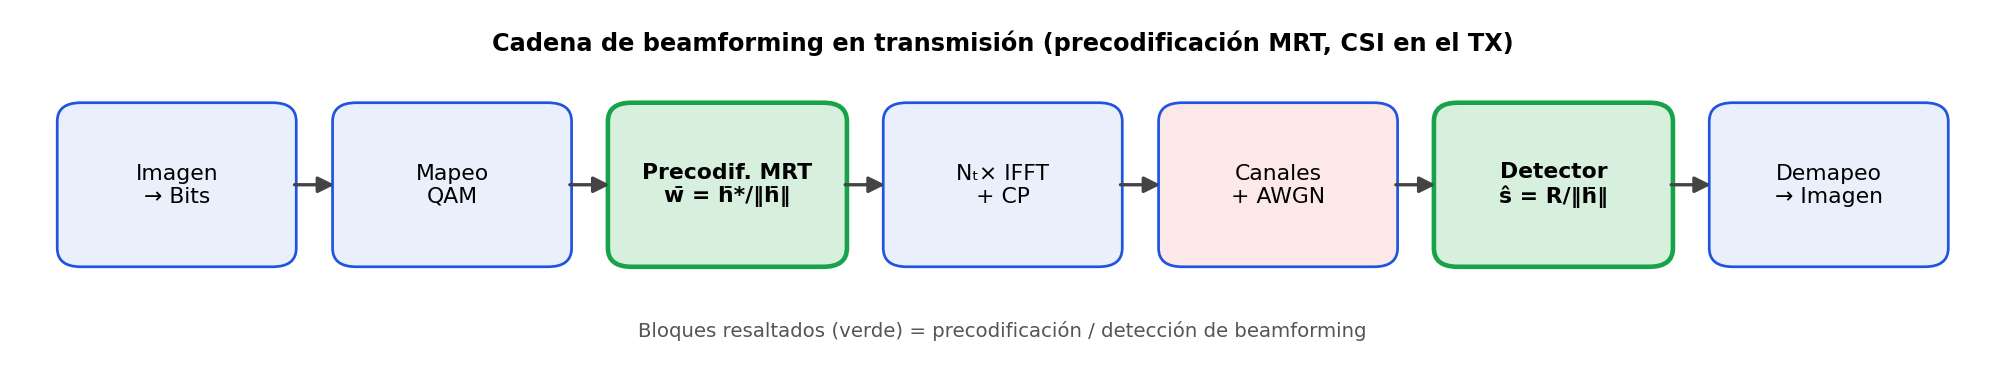
\includegraphics[width=0.95\textwidth]{img/diagrama_bf.png}
\caption{Diagrama de bloques de la cadena de beamforming; se resaltan el precodificador MRT $\bar v=\bar h^{*}/\|\bar h\|$ y el detector $\hat s=R/\|\bar h\|$, los bloques que la diferencian del transmisor OFDM de una sola antena.}
\label{fig:diagrama}
\end{figure}

\section{Evaluaci\'on -- An\'alisis de resultados}

En esta secci\'on se describen los par\'ametros de configuraci\'on; se examinan transmisiones de imagen con $2\times1$ y $4\times1$; se inspecciona la constelaci\'on recibida sin beamforming frente a MRT; y se caracteriza la ganancia mediante las curvas de BER frente a SNR (Monte Carlo), que constituyen el resultado central. La configuraci\'on empleada es $BW{=}5$~MHz, $\Delta f{=}15$~kHz y CP normal.

\subsection{Interfaz y par\'ametros de configuraci\'on}

La Fig.~\ref{fig:params} resume los par\'ametros derivados: $N_{SC}=300$ subportadoras, $N_{FFT}=512$, $f_s=7{,}680$~MHz y $N_{CP}=36$ muestras. Como en SFBC, el beamforming no intercala pilotos: toda la rejilla transporta datos y el canal se conoce de forma \textit{genie}. La precodificaci\'on se aplica de forma independiente sobre las $300$ subportadoras.

\begin{figure}[H]
\centering
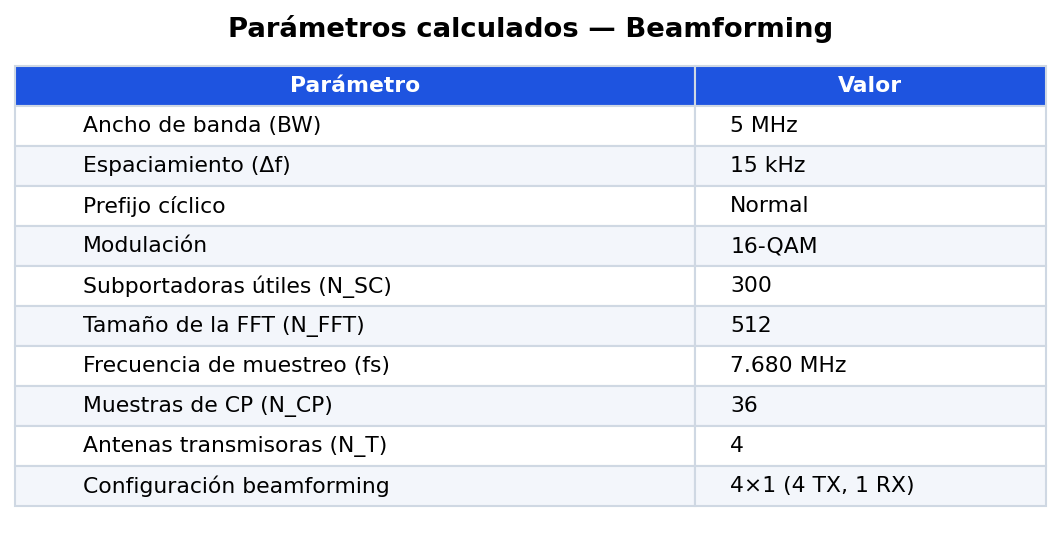
\includegraphics[width=0.6\textwidth]{img/params_bf.png}
\caption{Par\'ametros calculados para beamforming ($BW{=}5$~MHz, $\Delta f{=}15$~kHz, CP normal): $N_{SC}{=}300$, $N_{FFT}{=}512$ y configuraci\'on seleccionada.}
\label{fig:params}
\end{figure}

\subsection{Transmisi\'on de im\'agenes con beamforming}

Se transmiti\'o la misma imagen de prueba ($256\times256$ p\'ixeles, $1311$ s\'imbolos OFDM) con 16-QAM y SNR de $12$~dB. Sin beamforming ($1\times1$) la BER es $5{,}43\times10^{-2}$. Con beamforming $2\times1$ (Fig.~\ref{fig:sim2x1}) la imagen se recupera con un moteado leve y una BER de $1{,}04\times10^{-2}$, y con $4\times1$ (Fig.~\ref{fig:sim4x1}) la imagen es pr\'acticamente id\'entica a la original, con una BER de $5{,}2\times10^{-4}$ ---dos \'ordenes de magnitud por debajo del caso sin beamforming--- gracias a la ganancia combinada de arreglo y diversidad. La Tabla~\ref{tab:sims} resume estos resultados.

\begin{table}[H]
\centering
\caption{Resultados de las transmisiones de imagen con beamforming (16-QAM, SNR${=}12$~dB).}
\label{tab:sims}
\begin{tabular}{|l|c|c|c|}
\hline
\textbf{Configuraci\'on} & \textbf{Orden div.} & \textbf{BER} & \textbf{S\'imb. OFDM} \\
\hline
Sin beamforming ($1\times1$) & $1$ & $5{,}43\times10^{-2}$ & $1311$ \\
Beamforming $2\times1$       & $2$ & $1{,}04\times10^{-2}$ & $1311$ \\
Beamforming $4\times1$       & $4$ & $5{,}2\times10^{-4}$  & $1311$ \\
\hline
\end{tabular}
\end{table}

\begin{figure}[H]
\centering
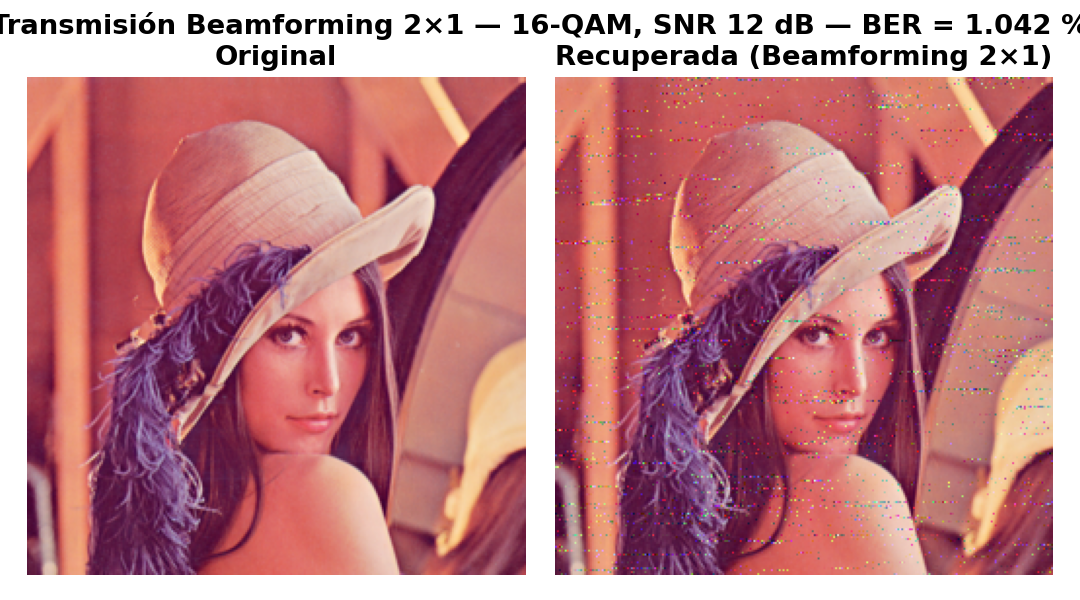
\includegraphics[width=0.6\textwidth]{img/sim_2x1_bf.png}
\caption{Transmisi\'on beamforming $2\times1$ con 16-QAM y SNR${=}12$~dB. La imagen recuperada presenta un moteado leve (BER ${=}1{,}04\times10^{-2}$).}
\label{fig:sim2x1}
\end{figure}

\begin{figure}[H]
\centering
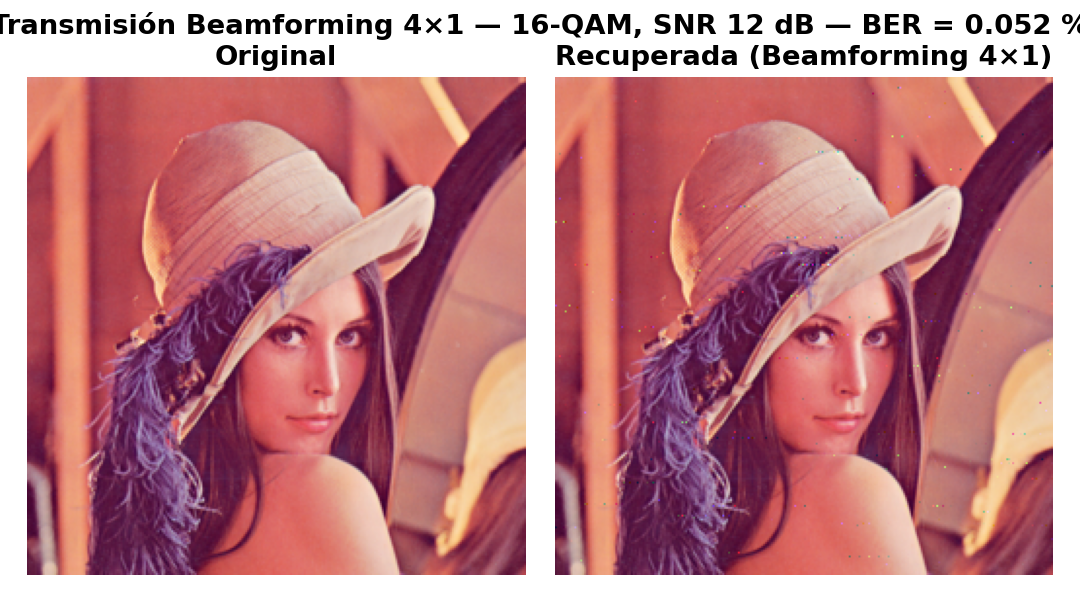
\includegraphics[width=0.6\textwidth]{img/sim_4x1_bf.png}
\caption{Transmisi\'on beamforming $4\times1$ con 16-QAM y SNR${=}12$~dB. La imagen recuperada es pr\'acticamente id\'entica a la original (BER ${=}5{,}2\times10^{-4}$).}
\label{fig:sim4x1}
\end{figure}

\subsection{Constelaci\'on recibida: sin beamforming frente a MRT}

La Fig.~\ref{fig:const} compara la constelaci\'on de 16-QAM recibida sin beamforming ($1\times1$, izquierda) y con beamforming $4\times1$ (derecha) a $15$~dB. En el caso $1\times1$ los s\'imbolos aparecen muy dispersos por los desvanecimientos del canal, que la ecualizaci\'on Zero-Forcing de una sola antena no puede corregir. Con beamforming la nube se compacta fuertemente en torno a las posiciones ideales de la ret\'icula: la precodificaci\'on suma en fase la energ\'ia de las cuatro antenas \eqref{eq:recibido}, elevando la SNR efectiva (ganancia de arreglo) y reduciendo la probabilidad de un desvanecimiento simult\'aneo (diversidad). Es la manifestaci\'on visual directa de la ganancia obtenida.

\begin{figure}[H]
\centering
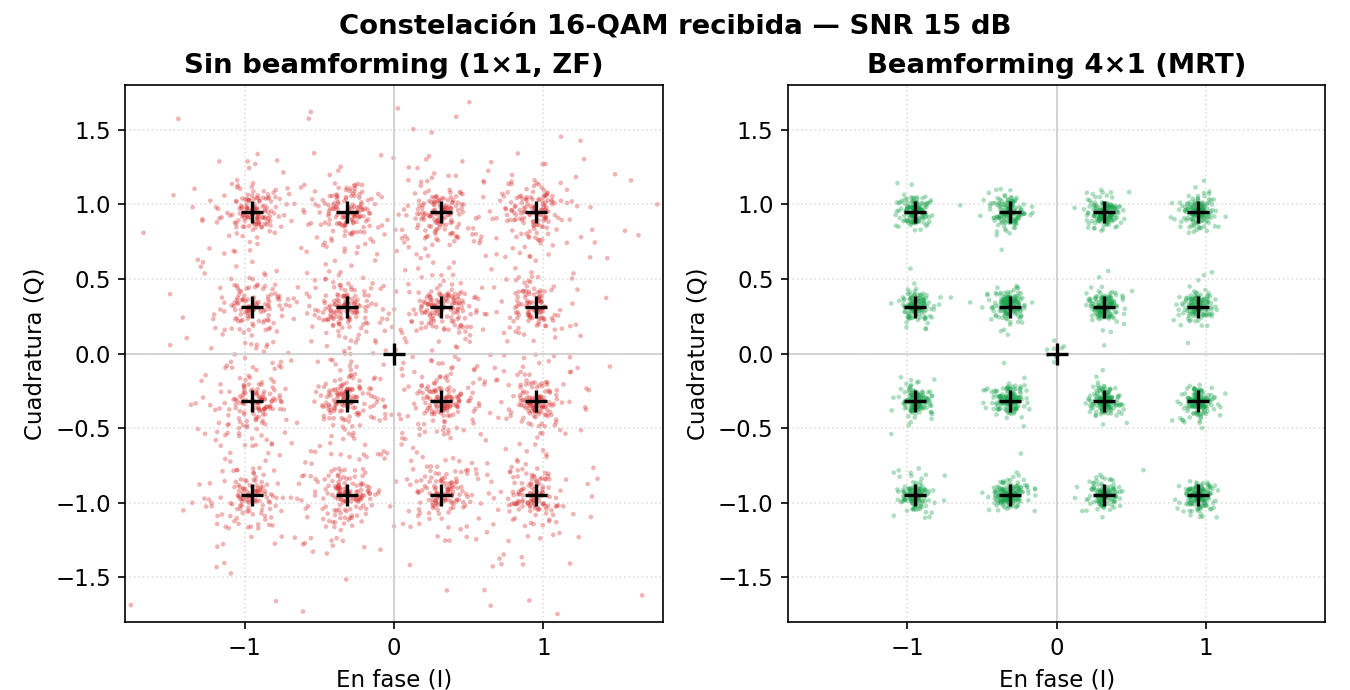
\includegraphics[width=0.95\textwidth]{img/constelacion_bf.png}
\caption{Constelaci\'on de 16-QAM recibida a $15$~dB: sin beamforming ($1\times1$, izquierda, dispersa) frente a beamforming $4\times1$ (derecha, compacta).}
\label{fig:const}
\end{figure}

\subsection{Curvas BER frente a SNR (Monte Carlo): resultado central}

La Fig.~\ref{fig:montecarlo} superpone las tres curvas de BER frente a SNR de los \'ordenes de beamforming ($1\times1$, $2\times1$, $4\times1$) con $8$ corridas por punto e IC al $95\%$ para 16-QAM. Las curvas exhiben \emph{pendientes claramente distintas} correspondientes a los \'ordenes de diversidad $1$, $2$ y $4$, y se corren a la izquierda al aumentar $N_T$ por la ganancia de arreglo. La Tabla~\ref{tab:ber} recoge valores representativos: a $15$~dB la BER pasa de $3{,}1\times10^{-2}$ sin beamforming a $3{,}6\times10^{-3}$ con $2\times1$ y a $1{,}0\times10^{-4}$ con $4\times1$, y la separaci\'on entre curvas se ensancha con la SNR, como predice la diferencia de pendientes.

\begin{table}[H]
\centering
\caption{BER frente a SNR (Monte Carlo, 16-QAM) para los \'ordenes de beamforming.}
\label{tab:ber}
\begin{tabular}{|c|c|c|c|}
\hline
\textbf{SNR (dB)} & \textbf{$1\times1$} & \textbf{BF $2\times1$} & \textbf{BF $4\times1$} \\
\hline
$6$  & $1{,}5\times10^{-1}$ & $6{,}6\times10^{-2}$ & $2{,}0\times10^{-2}$ \\
$9$  & $1{,}0\times10^{-1}$ & $3{,}4\times10^{-2}$ & $3{,}6\times10^{-3}$ \\
$12$ & $5{,}6\times10^{-2}$ & $1{,}1\times10^{-2}$ & $6{,}3\times10^{-4}$ \\
$15$ & $3{,}1\times10^{-2}$ & $3{,}6\times10^{-3}$ & $1{,}0\times10^{-4}$ \\
$18$ & $1{,}8\times10^{-2}$ & $1{,}1\times10^{-3}$ & $1{,}8\times10^{-5}$ \\
\hline
\end{tabular}
\end{table}

\begin{figure}[H]
\centering
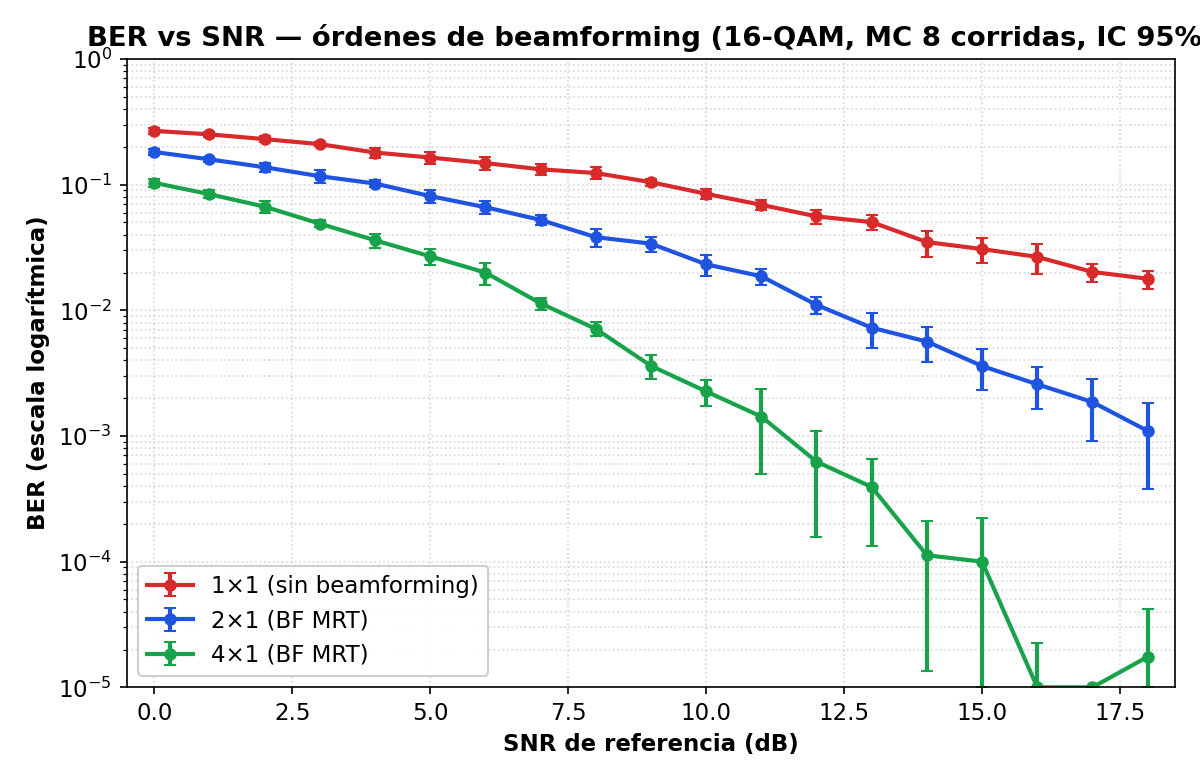
\includegraphics[width=0.9\textwidth]{img/montecarlo_bf.png}
\caption{BER frente a SNR (16-QAM): \'ordenes de beamforming $1\times1$, $2\times1$ y $4\times1$, Monte Carlo con $8$ corridas por punto e IC al $95\%$. Pendientes crecientes (diversidad) y corrimiento a la izquierda (ganancia de arreglo).}
\label{fig:montecarlo}
\end{figure}

\subsection{Comparaci\'on al orden 2: beamforming, SFBC y MRC}

La Fig.~\ref{fig:overlay} compara, al mismo orden de diversidad $2$, el beamforming $2\times1$ (con CSI en TX), el SFBC $2\times1$ (sin CSI en TX) y el MRC $1\times2$ (diversidad en recepci\'on), las tres sobre el mismo piso de ruido. Beamforming $2\times1$ y MRC $1\times2$ \emph{se solapan}, como corresponde a t\'ecnicas duales que combinan coherentemente la potencia completa, mientras que SFBC $2\times1$ queda cerca de $3$~dB por encima a igualdad de BER, penalizaci\'on que proviene de repartir la potencia entre las dos antenas \emph{a ciegas} por no disponer de informaci\'on del canal en el transmisor. La Tabla~\ref{tab:overlay} cuantifica esta diferencia: a $15$~dB, BF $2\times1$ y MRC $1\times2$ rondan $3$--$4\times10^{-3}$, frente a $1{,}0\times10^{-2}$ de SFBC.

\begin{table}[H]
\centering
\caption{BER frente a SNR (Monte Carlo, 16-QAM) al orden de diversidad 2.}
\label{tab:overlay}
\begin{tabular}{|c|c|c|c|}
\hline
\textbf{SNR (dB)} & \textbf{BF $2\times1$} & \textbf{MRC $1\times2$} & \textbf{SFBC $2\times1$} \\
\hline
$6$  & $6{,}6\times10^{-2}$ & $6{,}9\times10^{-2}$ & $1{,}2\times10^{-1}$ \\
$9$  & $3{,}4\times10^{-2}$ & $3{,}4\times10^{-2}$ & $6{,}0\times10^{-2}$ \\
$12$ & $1{,}1\times10^{-2}$ & $1{,}1\times10^{-2}$ & $2{,}8\times10^{-2}$ \\
$15$ & $3{,}6\times10^{-3}$ & $4{,}2\times10^{-3}$ & $1{,}0\times10^{-2}$ \\
$18$ & $1{,}1\times10^{-3}$ & $1{,}6\times10^{-3}$ & $3{,}4\times10^{-3}$ \\
\hline
\end{tabular}
\end{table}

\begin{figure}[H]
\centering
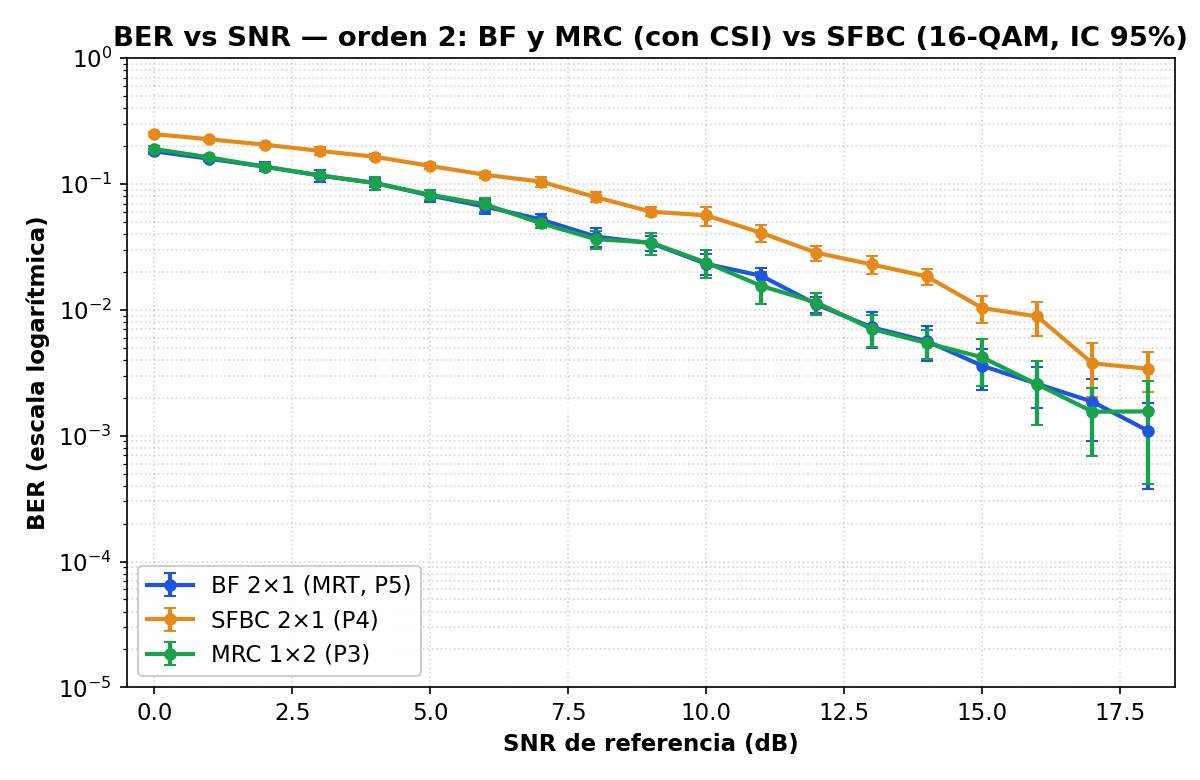
\includegraphics[width=0.9\textwidth]{img/montecarlo_overlay.png}
\caption{BER frente a SNR (16-QAM) al orden de diversidad 2: beamforming $2\times1$ y MRC $1\times2$ (con CSI) se solapan y superan en $\sim3$~dB a SFBC $2\times1$ (sin CSI en TX).}
\label{fig:overlay}
\end{figure}

\section{Conclusiones}

Se implement\'o y evalu\'o el beamforming en transmisi\'on mediante el vector de precodificaci\'on MRT $\bar v=\bar h^{*}/\|\bar h\|$ descrito en las diapositivas del curso \cite{vazquez_cmoviles}, reutilizando \'integramente la cadena OFDM de las pr\'acticas anteriores. La incorporaci\'on requiri\'o \'unicamente dos elementos espec\'ificos ---el precodificador MRT por subportadora y su detector---, lo que confirma que el esquema se integra de forma natural sobre OFDM al precodificar de manera independiente cada subportadora plana.

Los resultados verifican el objetivo. El an\'alisis de Monte Carlo mostr\'o que las curvas de los \'ordenes $1\times1$, $2\times1$ y $4\times1$ presentan pendientes crecientes acordes con los \'ordenes de diversidad $1$, $2$ y $4$, y un corrimiento a la izquierda al a\~nadir antenas, reflejo de la \emph{ganancia de arreglo} que anticipan las diapositivas (potencia recibida proporcional a $N_T$). La transmisi\'on de im\'agenes y las constelaciones confirmaron visualmente esta mejora. Finalmente, la comparaci\'on al orden $2$ evidenci\'o que beamforming $2\times1$ y MRC $1\times2$ se solapan ---son t\'ecnicas duales--- y superan en cerca de $3$~dB a SFBC $2\times1$: contar con conocimiento del canal en el transmisor permite combinar la potencia coherentemente, mientras que SFBC debe repartirla a ciegas. Esta ventaja, junto con el hecho de mantener una sola antena en el terminal, es la raz\'on por la que LTE adopta el beamforming basado en precodificaci\'on en el enlace descendente.

\bibliographystyle{IEEEtran}
\bibliography{referencias}

\clearpage
\onecolumn
\newpage
\section*{Anexos}

\begin{figure}[H]
    \centering
    
\includegraphics[width=0.22\textwidth]{img/qr_sitio.png}
    \caption{C\'odigo QR del simulador desplegado: \texttt{https://ofdm.tesisucuenca.com}}
    \label{fig:qrsitio}
\end{figure}

\begin{figure}[H]
    \centering
    
\includegraphics[width=0.22\textwidth]{img/qr_repo.png}
    \caption{C\'odigo QR del repositorio del proyecto: \texttt{https://github.com/thyron001/ofdm}}
    \label{fig:qrrepo}
\end{figure}

\end{document}
